%%%%%%%%%%%%%%%%%%%%%%%%%%%%%%%%%%%%%%%%%
% Beamer Presentation
% LaTeX Template
% Version 1.0 (10/11/12)
%
% This template has been downloaded from:
% http://www.LaTeXTemplates.com
%
% License:
% CC BY-NC-SA 3.0 (http://creativecommons.org/licenses/by-nc-sa/3.0/)
%
%%%%%%%%%%%%%%%%%%%%%%%%%%%%%%%%%%%%%%%%%

%----------------------------------------------------------------------------------------
%	PACKAGES AND THEMES
%----------------------------------------------------------------------------------------

\documentclass{beamer}

\mode<presentation> {

% The Beamer class comes with a number of default slide themes
% which change the colors and layouts of slides. Below this is a list
% of all the themes, uncomment each in turn to see what they look like.

%\usetheme{default}
%\usetheme{AnnArbor}
%\usetheme{Antibes}
%\usetheme{Bergen}
%\usetheme{Berkeley}
%\usetheme{Berlin}
%\usetheme{Boadilla}
%\usetheme{CambridgeUS}
%\usetheme{Copenhagen}
%\usetheme{Darmstadt}
%\usetheme{Dresden}
%\usetheme{Frankfurt}
%\usetheme{Goettingen}
%\usetheme{Hannover}
%\usetheme{Ilmenau}
%\usetheme{JuanLesPins}
%\usetheme{Luebeck}
\usetheme{Madrid}
%\usetheme{Malmoe}
%\usetheme{Marburg}
%\usetheme{Montpellier}
%\usetheme{PaloAlto}
%\usetheme{Pittsburgh}
%\usetheme{Rochester}
%\usetheme{Singapore}
%\usetheme{Szeged}
%\usetheme{Warsaw}

% As well as themes, the Beamer class has a number of color themes
% for any slide theme. Uncomment each of these in turn to see how it
% changes the colors of your current slide theme.

%\usecolortheme{albatross}
%\usecolortheme{beaver}
%\usecolortheme{beetle}
%\usecolortheme{crane}
%\usecolortheme{dolphin}
%\usecolortheme{dove}
%\usecolortheme{fly}
%\usecolortheme{lily}
%\usecolortheme{orchid}
%\usecolortheme{rose}
%\usecolortheme{seagull}
%\usecolortheme{seahorse}
%\usecolortheme{whale}
%\usecolortheme{wolverine}

%\setbeamertemplate{footline} % To remove the footer line in all slides uncomment this line
%\setbeamertemplate{footline}[page number] % To replace the footer line in all slides with a simple slide count uncomment this line

%\setbeamertemplate{navigation symbols}{} % To remove the navigation symbols from the bottom of all slides uncomment this line
}

\usepackage{graphicx} % Allows including images
\usepackage{booktabs} % Allows the use of \toprule, \midrule and \bottomrule in tables
\usepackage{hyperref} % Allows link in pdf


%----------------------------------------------------------------------------------------
%	TITLE PAGE
%----------------------------------------------------------------------------------------


\title[Information Extraction]{Information Extraction: A short introduction}

\author{Rafael Carrascosa}
\institute[\href{http://www.machinalis.com/}{Machinalis}] % Your institution as it will appear on the bottom of every slide, may be shorthand to save space
{
\href{http://www.machinalis.com/}{Machinalis} \\ % Your institution for the title page
\medskip
\textit{rcarrascosa@machinalis.com} % Your email address
}
\date{\today} % Date, can be changed to a custom date


\begin{document}

\begin{frame}
\titlepage % Print the title page as the first slide
\end{frame}

\begin{frame}
\frametitle{About the speaker}
\begin{itemize}
\item Rafael Carrascosa.
\item Background in Computer Science.
\item Works as developer and Machine Leaning specialist for Machinalis.
\item Machinalis (www.machinalis.com) is a software research and development company based on Argentina.
\item Leaded the delopment of IEPY.
\end{itemize}
\end{frame}


\begin{frame}
\frametitle{Overview} % Table of contents slide, comment this block out to remove it
\tableofcontents % Throughout your presentation, if you choose to use \section{} and \subsection{} commands, these will automatically be printed on this slide as an overview of your presentation
\end{frame}


%===================================
%===================================
%===================================
\section{Information Extraction}
%===================================
%===================================
%===================================


\subsection{What is IE?}

\begin{frame}
\frametitle{What is Information Extraction}

\vfill

\begin{block}{\centerline{In one line}}
    \centerline{Is about getting information from text automatically}
\end{block}

\vfill

\begin{itemize}
    \item Main activity: extract {\bf relation} instances between {\bf entities}.
    \item {\bf Entity}: Any-thing: A person, a place, an organization, a date, etc.
    \item {\bf Relation}: Can be any kind of linking concept between entities.
    \item Also posible but not common: IE over audio, images or video.
\end{itemize}

\end{frame}

%    \item It becomes necesary when:
%        \begin{itemize}
%            \item There are too much documents to read "by hand"
%            \
%        \end{itemize}


\begin{frame}
\frametitle{An example of entities and relations}

\begin{block}{Example text}
    {\bf Harvard University} is a private Ivy League research university in
    {\bf Cambridge}, Massachusetts, established 1636.
\end{block}

\begin{itemize}
    \item {\tt Harvard University}: Is an {\bf entity} of kind organization.
    \item {\tt Cambridge}: Is an {\bf entity} of kind location.
    \item $Located(X, Y)$ is a {\bf relation} that links organizations with places.
\end{itemize}

\pause

\begin{block}{ }
IE deals with detecting that
\[Located(\text{Harvard University}, \text{Cambridge})\]
is a {\bf relation instance} in the text.
\end{block}


\end{frame}


%\begin{frame}
%\frametitle{An example of entities and relations}

%\begin{block}{ }
%    {\bf John von Neumann} ({\bf December 28, 1903} – February 8, 1957) was a
%    Hungarian and American pure and applied mathematician, physicist, inventor
%    and polymath.
%\end{block}

%\begin{itemize}
%    \item Entity 1: {\bf \tt John von Neumann}
%    \item Entity 2: {\bf \tt December 28, 1903}
%    \item Relation instance: {\tt John von Neumann {\bf was born in} December 28, 1903}
%\end{itemize}

%\end{frame}

\subsection{Applications of IE}

\begin{frame}
\frametitle{Example application: Protests}

\pause

\begin{block}{ }
Use news text to build a map of events like politic acts or public protests.
\end{block}

\pause

\begin{itemize}
 \item News sites, social networks
 \item $happened\_at(protest, date)$
 \item $happened\_in(protest, location)$
 \item Data can end up in a map, or a timeline.
\end{itemize}

\end{frame}


\begin{frame}
\frametitle{Example application: Foodborne outbreaks}

\begin{block}{ }
Use social media comments to detect foodborne outbreaks.
\end{block}

\pause

\begin{itemize}
 \item $ate\_at(person, restaurant)$
 \item $has\_symptom(person, symptom)$
 \item True story: a colaboration between Yelp, Columbia University and NYC's
       Department of Health and Mental Hygiene.
\end{itemize}

\end{frame}

\begin{frame}
\frametitle{More example applications}

\begin{itemize}
 \item Starting from business news build a network graph with deals, investments, acquisitions.
 \item With sanitary documents, build a timeline of diseases, symptoms and treatments.
 \item Reconstructing state terrorism victims' fate from military documents.
 \item Use social media to measure the growth of statup incubators and co-working spaces.
 \item \dots
\end{itemize}

\end{frame}

\subsection{Limitations of IE}

%COMMENT No IE system is going to do what you need out-of-the-box, you will
% always need to tune it to your domain.

\begin{frame}
\frametitle{What is not IE}

\pause

\vfill
\begin{block}{ }
\centerline{Is not relation discovery, relations have to be known a-priori.}
\end{block}
\pause
\vfill
\begin{block}{ }
\centerline{Is not open domain, IE is domain specific.}
\end{block}
\vfill

\end{frame}


\subsection{How IE is done, a sketch}


%Entity stuff: the sofistication of this stage has impact later on
%Rel. ext.: Core problem of IE

\begin{frame}
\frametitle{A sketch of an IE system}

\begin{block}{Steps}
\begin{itemize}
    \item Basic natural language processing
    \item Entity recognition and linking
    \begin{itemize}
        \item<2-> Named entity recognition
        \item<2-> Coreference resolution
        \item<2-> Name linking
    \end{itemize}
    \item Relation extraction
    \begin{itemize}
        \item<3-> Rule-based
        \item<3-> Corpus-based
    \end{itemize}
\end{itemize}
\end{block}

\end{frame}


\begin{frame}
\frametitle{Relation extraction}

\begin{block}{Rule-based}
A regular expression to detect the presence of a relation.
\begin{itemize}
    \item Handcrafted by an expert
    \item Suggested and validated by an algorithm
\end{itemize}
\end{block}

\begin{block}{Corpus-based}
For each pair of entities, a binary classification:
\begin{itemize}
    \item Classifiers: Naive bayes, support vector machines, etc.
    \item Language models: Markov models, conditional random fields, etc.
\end{itemize}
\end{block}

\end{frame}

%The choice of the approach strongly influences the way the tool is going to
%be used and the performance characteristics you can expect.

%Rule: Requires experts with a systematic understanding of the domain.
%      Expect high precision, low recall.
%Stat: Requires only casual understanding of the domain.
%      Tuneable precision vs recall tradeoff.

\subsection{Reasoning and Knowledge Bases}

% Two more things that give relevancy to IE

\begin{frame}
\frametitle{Knowledge Bases and Reasoning}

\begin{block}{Knowledge bases}
\begin{itemize}
\item Freebase  % TODO: Links?
\item Linked open data   % TODO : Links?
\end{itemize}
\end{block}

\pause

\begin{block}{Reasoning}
Semantic reasoners, they exist.  % OWL, Jena, Semantic web
\end{block}

\end{frame}



\begin{frame}
\frametitle{IE summary}

\begin{itemize}
    \item Getting information out of large amounts of text documents.
    \item Extract {\bf relation} instances between {\bf entities}.
    \item Has many practical applications.
    \item Domain-specific.
    \item Solved using rules or statistic tools.
\end{itemize}

\end{frame}


%===================================
%===================================
%===================================
\section{IE with IEPY}
%===================================
%===================================
%===================================


\subsection{Overview}

\begin{frame}
\frametitle{IE with IEPY}
\huge{\centerline{IE with IEPY}}
\end{frame}

\begin{frame}
\frametitle{What is IEPY}

\begin{itemize}
\item Tool for Information Extraction.
\item Open source (BSD).
\item Written in Python.
\item Developed by Machinalis.
\item Aimed at:
\begin{itemize}
    \item IE users
    \item IE scientists
\end{itemize}
\item {\tt https://github.com/machinalis/iepy}
\end{itemize}
\end{frame}

% Users: Needing to perform Information Extraction on a large dataset.
% Scientists: wanting to experiment with new IE algorithms.


\begin{frame}
\frametitle{Features}
    
\begin{block}{For IE users}
    \begin{itemize}
        \item NER and coreference resolution.
        \item {\bf Active learning} relation extraction.  % Pre-configured with good defaults
        \item {\bf Rule-based relation extraction}. % For cases where the documents are semi-structured or high precision is required.
    \end{itemize}
\end{block}
\begin{block}{For IE scientists}
    \begin{itemize}
        \item {\bf Corpus annotation} tool.
        \item Web-based UI. % that allows decentralized human input.
        \item Easily hackable.  % ideal for scientist wanting to experiment with new algorithms.
    \end{itemize}
\end{block}

\end{frame}


\subsection{Relation extraction with IEPY}


\begin{frame}
\frametitle{IEPY: Active learning core}

\begin{block}{Statistical classifier}
\begin{itemize}
 \item Support Vector Machine (by default).
 \item Features: Bag-of-words, POS tags, entity distance, etc.
 \item Active learning.
 \item Tunable to high-precision or high-recall.
 \item Web-based UI to interact with the expert.
 \item Easily hackable ({\tt scikit-klearn} and {\tt django}) 
\end{itemize}
\end{block}
\end{frame}

\begin{frame}
\frametitle{IEPY: Active learning core}

\begin{block}{Active learning goal}
    \centerline{Minimize human effort}
\end{block}

\pause
\begin{block}{Idea}
\begin{itemize}
    \item Query a human expert.
    \item Use the answer to compute the next most useful questions to ask.
    \item Repeat.
\end{itemize}
\end{block}

Uses less human time to achieve the same performance.

\end{frame}

\begin{frame}
\frametitle{IEPY: Active learning core}

\begin{figure}
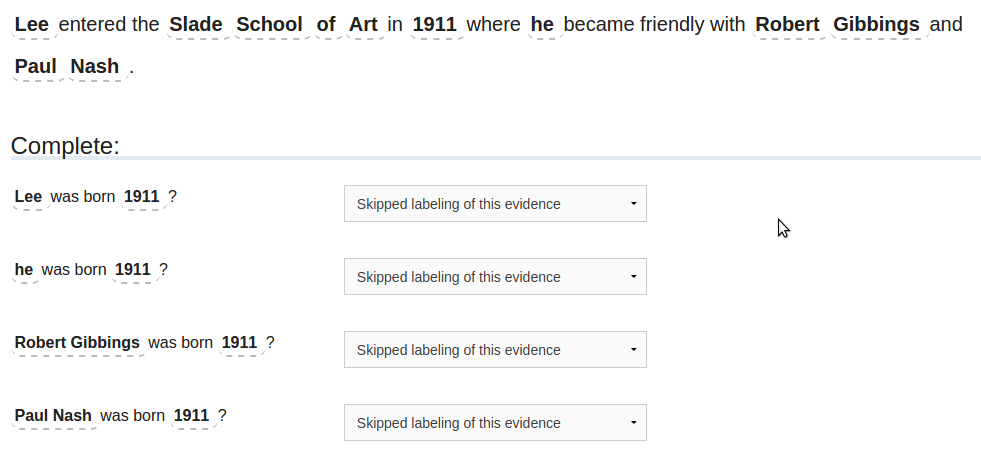
\includegraphics[width=1\linewidth]{al1}
\end{figure}

\end{frame}

%Webui: Allows multiple experts to work simultaneously.
%       Is far more friendly than a console program or a spreadsheet,
%       allowing experts which don't know much about computers to easily participate


\begin{frame}
\frametitle{IEPY: Rule core}

\begin{block}{Rule-based}
\begin{itemize}
 \item Enhanced regular expressions.
 \item Expresiveness: Words, POS tags, entities, entity kinds, etc.
 \item Positive or negative rules.
 \item Have to be written in Python.
 \item Simplified syntax
\end{itemize}
\end{block}

\end{frame}


\begin{frame}
\frametitle{Rule-based}

\begin{figure}
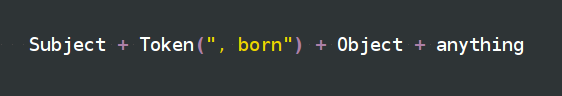
\includegraphics[scale=0.5]{rule1}
\end{figure}

\pause

\begin{block}{Matches something like}
\vspace{15pt}
{\bf Lyle Eugene Hollister}, born {\bf 6 July 1923} in Sioux Falls...
\vspace{15pt}
\end{block}

\end{frame}


\begin{frame}
\frametitle{Rule-based}

\begin{figure}
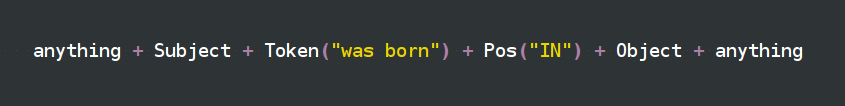
\includegraphics[width=1\linewidth]{rule2}
\end{figure}

\pause

\begin{block}{Matches something like}
\vspace{15pt}
\dots {\bf Shamsher M. Chowdhury} was born in {\bf 1950} \dots
\vspace{15pt}
\end{block}

\end{frame}


\subsection{Corpora construction}

\begin{frame}
\frametitle{Corpora construction}

\begin{block}{Evaluation?}
\vspace{15pt}
\centerline{Eventually you'll need to evaluate your IE performance.}
\vspace{15pt}
\pause

\begin{itemize}
  \item How much noise has the information you extracted?
  \item How many relevant facts you are leaving behind?
\end{itemize}

\end{block}


\end{frame}

\begin{frame}
\frametitle{Corpora construction}

IEPY has a corpora construction tool

\begin{figure}
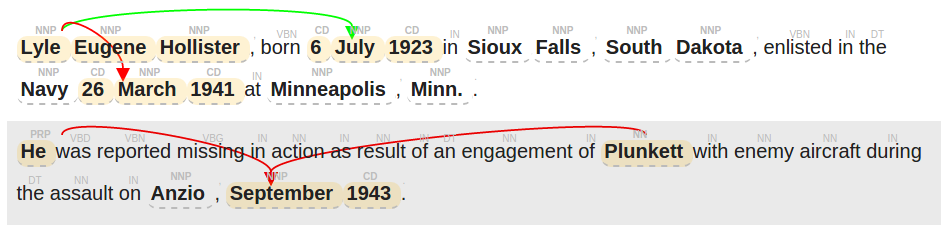
\includegraphics[width=1\linewidth]{corpora2}
\end{figure}

Since is a web-based it allows multiple experts to work simultaneously

\end{frame}


\begin{frame}
\frametitle{Some performance figures}

\begin{block}{Active learning}
On an easy relation (date of birth)
\[ 86\text{\% prec. and } 80\text{\% rec. }\]
with an hour's worth of labeling.
\end{block}

\begin{block}{Rule based}
On an easy relation (date of birth)
\[ 98.65\text{\% prec. and } 38\text{\% rec. }\]
investing 4 hours (11 rules).
\end{block}

\begin{block}{Corpora construction}
Rate of 50 documents per hour (we labeled 4300 docs).
\end{block}

% Name that we're publishing this corpus perdate and orgloc.

% Tunable to 95% prec and 35% recall

% On a harder relation: 71% precision (+-5%), 58% recall (+-6%) with 3 hours

\end{frame}


\begin{frame}
\frametitle{The end}

\Huge{\centerline{That's it, thank you!}}

\end{frame}


\end{document} 
